%% LaTeX-Beamer template for KIT design
%% by Erik Burger, Christian Hammer
%% title picture by Klaus Krogmann
%%
%% version 2.1
%%
%% mostly compatible to KIT corporate design v2.0
%% http://intranet.kit.edu/gestaltungsrichtlinien.php
%%
%% Problems, bugs and comments to
%% burger@kit.edu

\documentclass[18pt]{beamer}

%% SLIDE FORMAT

% use 'beamerthemekit' for standard 4:3 ratio
% for widescreen slides (16:9), use 'beamerthemekitwide'
% for widescreen slide without sidebar use 'beamerthemekitwidenosidebar'

\usepackage{xkeyval}
\usepackage{todonotes}
\presetkeys{todonotes}{inline}{}
\usepackage{templates/beamerthemekit}
%\usepackage{templates/beamerthemekitwide}
%\usepackage{templates/beamerthemekitwidenosidebar}

% use this to disable the latex beamer navigation symbols
%\beamertemplatenavigationsymbolsempty


%% TITLE PICTURE

% if a custom picture is to be used on the title page, copy it into the 'logos'
% directory, in the line below, replace 'mypicture' with the 
% filename (without extension) and uncomment the following line
% (picture proportions: 63 : 20 for standard, 169 : 40 for wide
% *.eps format if you use latex+dvips+ps2pdf, 
% *.jpg/*.png/*.pdf if you use pdflatex)

%\titleimage{mypicture}

%% TITLE LOGO

% for a custom logo on the front page, copy your file into the 'logos'
% directory, insert the filename in the line below and uncomment it

\titlelogo{2_TecO_Logo_m}

% (*.eps format if you use latex+dvips+ps2pdf,
% *.jpg/*.png/*.pdf if you use pdflatex)

%% TikZ INTEGRATION

% use these packages for PCM symbols and UML classes
% \usepackage{templates/tikzkit}
% \usepackage{templates/tikzuml}

% the presentation starts here

\title[]{Klassifikation von respiratorischen Ereignissen mit \\ Earables und maschinellem Lernen}
\subtitle{}
\author{David Laubenstein}

\institute{Institut für Telematik: Pervasive Computing Systems / TECO}

% Bibliography

\usepackage[citestyle=authoryear,bibstyle=numeric,hyperref,backend=biber]{biblatex}
\addbibresource{templates/example.bib}
\bibhang1em

\begin{document}

% change the following line to "ngerman" for German style date and logos
\selectlanguage{english}

%title page
\begin{frame}
\titlepage
\end{frame}

%table of contents
\begin{frame}{Outline/Gliederung}
\tableofcontents
\end{frame}

\section{Grundlagen}
\subsection{Problem}
\begin{frame}{Problem}
    \includegraphics[scale=0.4]{../Proposal/logos/was-passiert-bei-schlafapnoe}
\end{frame}

\begin{frame}{Problem}
%insert picture from sleeping labor
    \includegraphics[scale=0.12]{../Proposal/logos/sleepLabor}
\end{frame}

\subsection{Idee}
\begin{frame}{Idee}
%insert picture from Earbuds for solution to diagnose this 
    \begin{columns}[T] % align columns
	\begin{column}{.48\textwidth}
	    \includegraphics[scale=0.15]{../Proposal/logos/esense}
	\end{column}%
	\hfill%
	\begin{column}{.48\textwidth}
	    \includegraphics[scale=0.25]{../Proposal/logos/esense2}
	\end{column}%
	\end{columns}
	Vorteil:
	\begin{itemize}
		\item Test kann unkompliziert zuhause durchgeführt werden
		\item Sensoren bereits heute in Kopfhörern vorhanden (Apple AirPods)
	\end{itemize}
\end{frame}

\subsection{Idee}
\begin{frame}{Idee}
\begin{itemize}
\item Erstellung eines Datensatzes zur Klassifikation
\begin{itemize}
    \item eSense-Earpods mit IMU
\end{itemize}
\item Ground-Truth: Polysomnographie-Gerät
\item \todo{add pictures of Earables and psg}
\end{itemize}
\end{frame}

\section{Ablauf}
\begin{frame}{Ablauf}
\begin{itemize}
    \item 3 Schritte
    \begin{itemize}
        \item App
        \item Nutzerstudie $/$ Datensatz
        \item Analyse
    \end{itemize}
\end{itemize}
\end{frame}

\section{Nutzerstudie}
\begin{frame}{Nutzerstudie$/$ Datensatz}
\begin{itemize}
    \item Nutzerstudie
    \begin{itemize}
        \item 7 Personen 
        \item 3 Positionen (Bauch, Seite, Rücken)
    \end{itemize}
    \item Was wird aufgezeichnet?
    \begin{itemize}
        \item eSense-Earpods (\textbf{IMU, Mikrofon})
        \item PSG-System, 11 Sensoren, unter anderem:
        \begin{itemize}
            \item Pulssensor am Finger
            \item \dots \todo{fill with rest of sensors}
        \end{itemize}
    \end{itemize}
\end{itemize}
\end{frame}

\begin{frame}{Ablauf der Nutzerstudie}
    \includegraphics[scale=0.45]{images/study/study_flow2.pdf}
\end{frame}

\begin{frame}{Ablauf der Nutzerstudie}
    %\includegraphics[0.25]{images/study/study_flow2.pdf}
    \begin{center}
        \begin{columns}[T] % align columns
            \begin{column}{.33\textwidth}
                \centering
                \includegraphics[scale=0.1]{images/app/connect_success.PNG}
            \end{column}%
            \hfill%
            \begin{column}{.33\textwidth}
                \centering
                \includegraphics[scale=0.1]{images/app/measurement_details.PNG}
            \end{column}%
            \hfill%
            \begin{column}{.33\textwidth}
                \centering
                \includegraphics[scale=0.1]{images/app/measurement_timer_02.png}
            \end{column}%
        \end{columns} 
    \end{center}
\end{frame}

\begin{frame}{Beispielbilder der Nutzerstudie}
    \begin{center}
        \begin{columns}[T]
            \begin{column}{.49\textwidth}
                \centering
                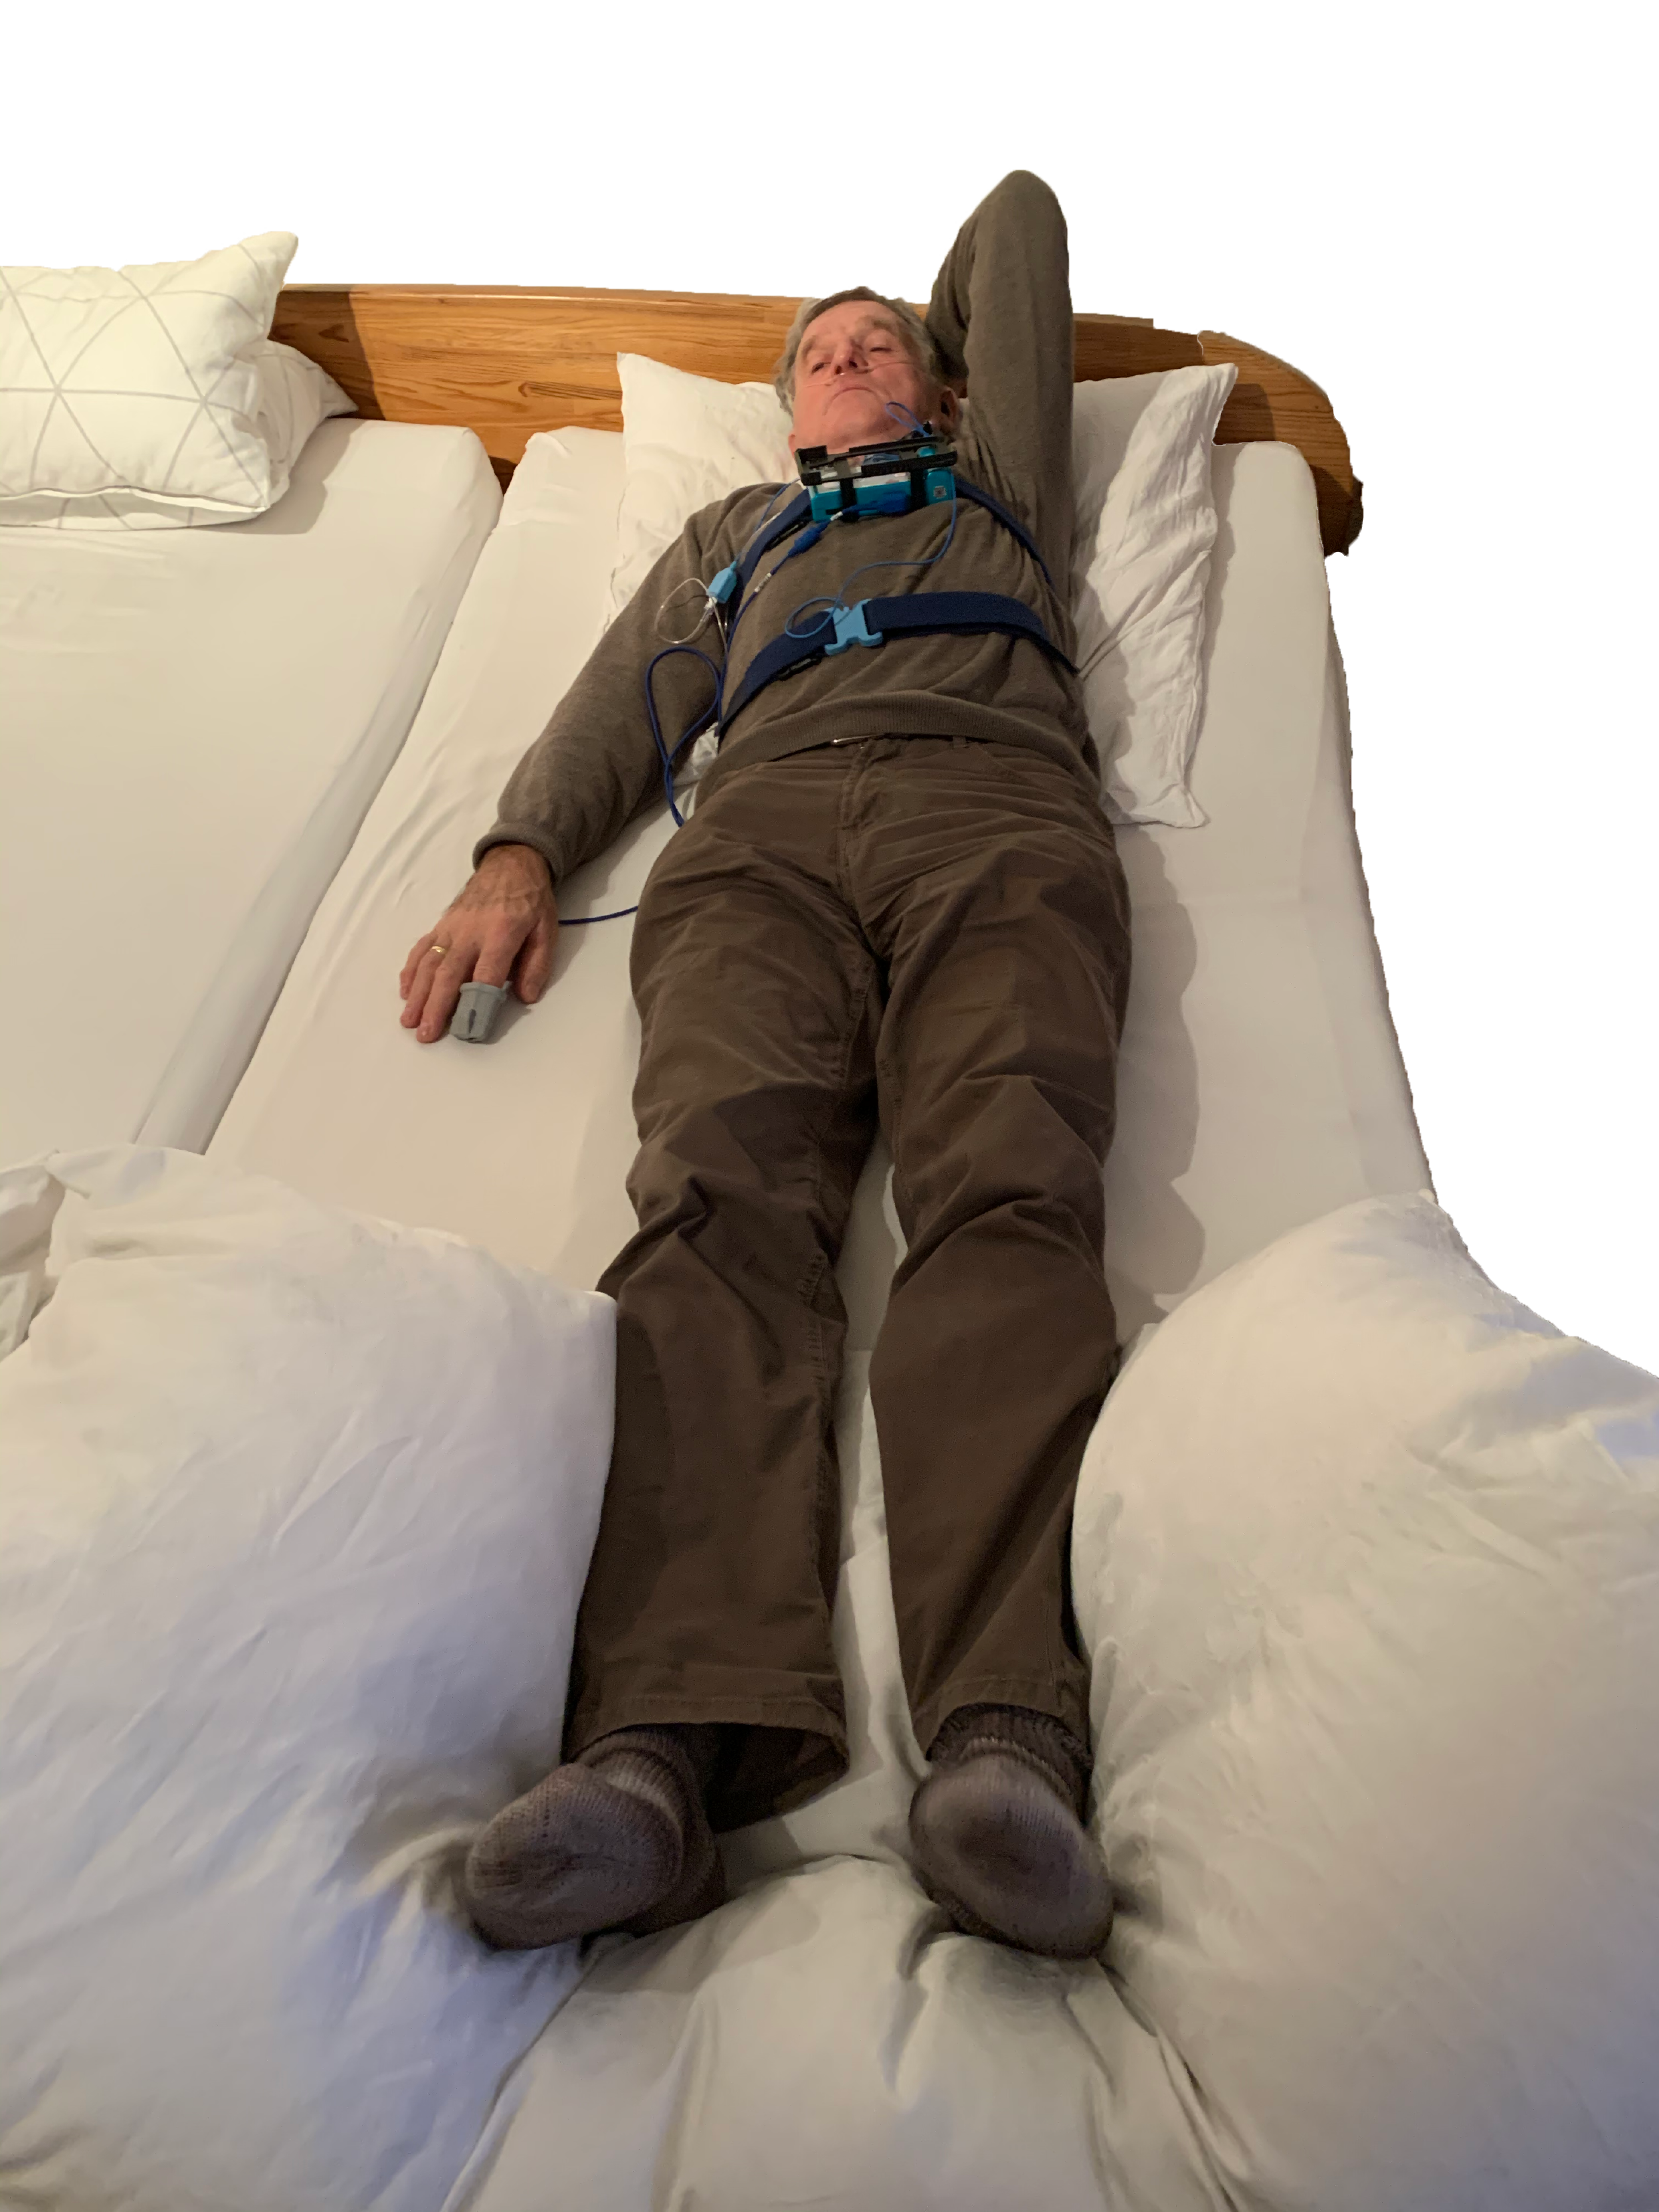
\includegraphics[scale=0.23]{images/study/study_proband_2_clean.png}
            \end{column}
            \hfill%
            \begin{column}{.49\textwidth}
                \centering
                \includegraphics[scale=0.12]{images/study/study_proband_clean2.png}
            \end{column}
        \end{columns}
    \end{center}
\end{frame}

\begin{frame}{Erste Resultate}
    \begin{center}
        \includegraphics[scale=0.16]{images/data_analyzation/compare_raw_signal_with_flowDr_2.png}
    \end{center}
\end{frame}

\section{Klassifikation}
\begin{frame}{Klassifikation / Idee}
\begin{itemize}
    \item Teile Messung in \textit{windows} auf
    \item Pro \textit{window} werden Features berechnet
    \item Klassifikation anhand der Features
    \begin{itemize}
        \item Evaluation mit dem Kreuzvalidierungsverfahren
        \begin{itemize}
            \item Within Subject
            \item Leave One Subject Out (LOSO)
        \end{itemize}
    \end{itemize}
\end{itemize}
\end{frame}

\begin{frame} {Leave One Subject Out}
    \begin{center}
        \includegraphics[scale=0.29]{images/evaluation/loso_10sec/xg_boost_loso/XGBoost(LeaveOneSubjectOutPerson6Back).png}
    \end{center}
    \begin{center}
        \includegraphics[scale=0.29]{images/evaluation/loso_10sec/xg_boost_loso/XGBoost(LeaveOneSubjectOutPerson6Side).png}
    \end{center}
    \begin{center}
        \includegraphics[scale=0.29]{images/evaluation/loso_10sec/xg_boost_loso/XGBoost(LeaveOneSubjectOutPerson6Stomach).png}
    \end{center}
\end{frame}

\begin{frame} {Leave One Subject Out}
    \begin{center}
        \includegraphics[scale=0.29]{images/evaluation/loso_10sec/xg_boost_loso/XGBoost(LeaveOneSubjectOutPerson8Back).png}
    \end{center}
    \begin{center}
        \includegraphics[scale=0.29]{images/evaluation/loso_10sec/xg_boost_loso/XGBoost(LeaveOneSubjectOutPerson8Side).png}
    \end{center}
    \begin{center}
        \includegraphics[scale=0.29]{images/evaluation/loso_10sec/xg_boost_loso/XGBoost(LeaveOneSubjectOutPerson8Stomach).png}
    \end{center}
\end{frame}

\section{Aussicht}
\begin{frame}{Potenzial / Aussicht}
    \todo{Puls und SPO2 mit  Pulsoxiometer}
    \todo{Klassifikation: Betrachtung vorangehender und nachfolgender \textit{windows}}
    \todo{Nutzerinformationen mit einbeziehen (Gewicht, Geschlecht)}
\end{frame}

\begin{frame} {Zusammenfassung}    
    \tableofcontents
\end{frame}

\appendix
\begin{frame}{test}
    \todo{Add test asdf}
\end{frame}
\beginbackup

\begin{frame}[allowframebreaks]{References}
\printbibliography
\end{frame}

\backupend

\end{document}
